\section{Spring Boot}\label{SpringInstal}

Wurde Docker erfolgreich installiert erfolgt nun die Anleitung zur Installation und Inbetriebnahme der Spring Boot Anwendung.
Die Installation zu Spring Boot ist recht einfach dazu benötigen wir lediglich das Java Developer Kit 1.8 und  Build-Management-Tool Maven.

\begin{enumerate}
    \item Die Installationsanwendung zu Java Developer Kit 1.8 kann unter folgendem Link aufgerufen werden:\\\href{https://www.oracle.com/java/technologies/javase-jdk8-downloads.html}{https://www.oracle.com/java/technologies/javase-jdk8-downloads.html}
    
    \item Im nächsten Schritt wird zunächst Maven heruntergeladen. Mit Maven kann man insbesondere Java-Programme standardisiert erstellen und verwalten. Den Link dazu finden Sie hier: \href{https://mirror.dkd.de/apache/maven/maven-3/3.6.3/binaries/apache-maven-3.6.3-bin.zip}{https://mirror.dkd.de/apache/maven/maven-3/3.6.3/binaries/apache-maven-3.6.3-bin.zip}.\\\\\textcolor{red}{Wichtig:} Es sollte darauf geachtet werden, dass die Binaries heruntergeladen werden. Diese enthalten einen Ordner mit der Bezeichnung "bin"{}, welcher für spätere Zwecke benötigt wird.
    
    \item Nachdem die Binaries heruntergeladen wurden, entpacken wir den Ordner. Da Maven jedes Mal wenn das Programm kompiliert werden soll benötigt wird, bietet es sich an den Ordner dauerhaft an einen "sicheren"{} Ort abzuspeichern. Es bietet sich an Maven in den Umgebungsvariable bekannt zu machen. Dadurch muss nicht bei jedem Maven-Befehl der korrekte Pfad zu den entpackten Ordner angegeben werden. Ist Maven dem System bekannt, wird wenn ein Maven-Befehl aufgerufen wird, der Pfad zum entpackten Ordner automatisch durch das System hinzugefügt.
    
    \item Nun öffnen Sie per Windows-Taste + Q das Suchfeld und suchen dort nach "{}Systemumgebungsvariablen bearbeiten"{} . Es sollte sich nun ein Fenster öffnen. Dort drücken Sie auf "Umgebungsvariablen bearbeiten"{}.
    
    \begin{center}
        \begin{minipage}[t]{0.5\textwidth}
            \centering
            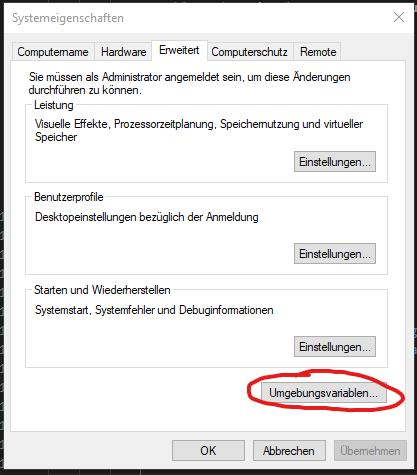
\includegraphics[width=(\textwidth)]{Kapitel3/SpringUmgebung.png}
            \captionof{figure}{Umgebungsvariable bearbeiten.}
            \label{ContainerConfig}
        \end{minipage}
    \end{center}

    \item Im nächsten Fenster wählen Sie zunächst unter Systemvariablen den Wert Path aus und drücken dann auf bearbeiten.
    
    \begin{center}
        \begin{minipage}[t]{0.5\textwidth}
            \centering
            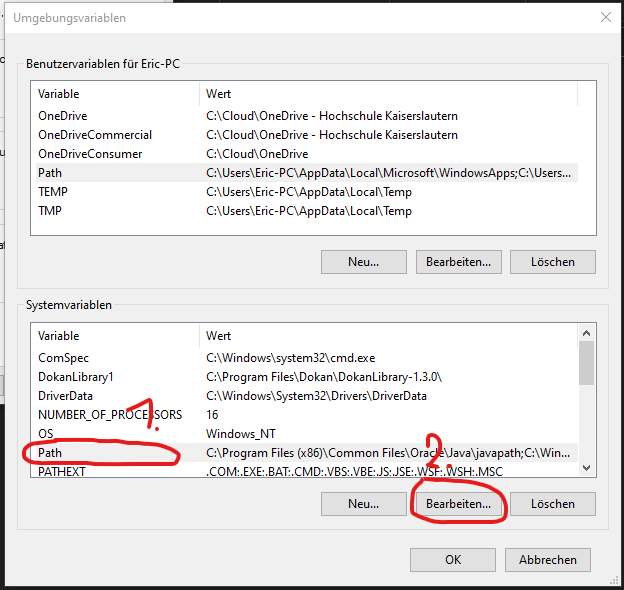
\includegraphics[width=(\textwidth)]{Kapitel3/SpringBearbeiten.png}
            \captionof{figure}{Umgebungsvariable bearbeiten.}
            \label{ContainerConfig}
        \end{minipage}
    \end{center}

    
    \item Dort fügen Sie mit "Neu"{} einen neuen Eintrag in der Tabelle hinzu und können nach auswählen der neuen Spalte über "Durchsuchen"{} den Pfad zu dem Maven-Ordner angeben.\\\\\textcolor{red}{Wichtig:} Zu beachten ist, dass der Ordner "bin"{} auf jeden Fall angegeben werden muss. Ansonsten kann Windows die benötigten Dateien nicht finden.

    \begin{center}
        \begin{minipage}[t]{0.5\textwidth}
            \centering
            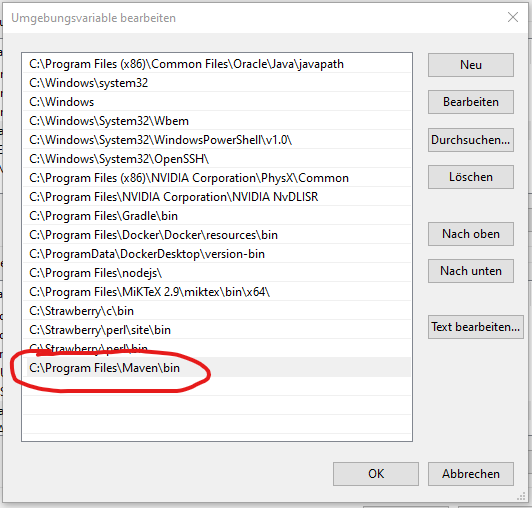
\includegraphics[width=(\textwidth)]{Kapitel3/SpringAdd.png}
            \captionof{figure}{Umgebungsvariable hinzufügen.}
            \label{ContainerConfig}
        \end{minipage}
    \end{center}
\end{enumerate}

